
\documentclass[12pt, a4paper, oneside, headinclude, footinclude]{article}

%----------------------------------------------------------------------------------------
%	REQUIRED PACKAGES
%----------------------------------------------------------------------------------------

\usepackage[
nochapters, 
beramono, 
eulermath,
pdfspacing, 
dottedtoc 
]{classicthesis} 

\usepackage{arsclassica} 
\usepackage{listings} 
\usepackage{minted} 
\usepackage[T1]{fontenc} 
\usepackage[utf8]{inputenc} 
\usepackage{graphicx} 
\graphicspath{{Figures/}} 
\usepackage{enumitem} 
\usepackage{lipsum} 
\usepackage{subfig} 
\usepackage{amsmath,amssymb,amsthm} 
\usepackage{varioref} 

%----------------------------------------------------------------------------------------
%	THEOREM STYLES
%---------------------------------------------------------------------------------------

\theoremstyle{definition} 
\newtheorem{definition}{Definition}

\theoremstyle{plain} 
\newtheorem{theorem}{Theorem}

\theoremstyle{remark} 

%----------------------------------------------------------------------------------------
%	HYPERLINKS
%---------------------------------------------------------------------------------------

\hypersetup{
colorlinks=true, breaklinks=true, bookmarks=true,bookmarksnumbered,
urlcolor=webbrown, linkcolor=RoyalBlue, citecolor=webgreen, 
pdftitle={}, 
pdfauthor={\textcopyright}, 
pdfsubject={}, 
pdfkeywords={}, 
pdfcreator={pdfLaTeX}, 
pdfproducer={LaTeX with hyperref and ClassicThesis} 
}


\title{\normalfont\spacedallcaps{Deep learning image analysis for disaster recovery, A DataKind report for the World Bank GFDRR}}

\author{\spacedlowsmallcaps{Patrick Doupe}} 

\date{} 

\begin{document}

\renewcommand{\sectionmark}[1]{\markright{\spacedlowsmallcaps{#1}}} 
\lehead{\mbox{\llap{\small\thepage\kern1em\color{halfgray} \vline}\color{halfgray}\hspace{0.5em}\rightmark\hfil}} 

\pagestyle{scrheadings} 

%----------------------------------------------------------------------------------------
%	TABLE OF CONTENTS & LISTS OF FIGURES AND TABLES
%----------------------------------------------------------------------------------------

\maketitle 

\setcounter{tocdepth}{2}

% \tableofcontents 

% \listoffigures 

% \listoftables

%----------------------------------------------------------------------------------------
%	ABSTRACT
%----------------------------------------------------------------------------------------

\section*{Abstract}

We discuss how the World Bank can use machine learning and satellite images to
improve disaster relief efforts. We include a review of image analysis with
convolutional neural networks. These networks are illustrated with code
examples using the \texttt{Keras} deep learning library. 

%----------------------------------------------------------------------------------------
%	AUTHOR AFFILIATIONS
%----------------------------------------------------------------------------------------

%\let\thefootnote\relax\footnotetext{* \textit{}}

%\let\thefootnote\relax\footnotetext{\textsuperscript{1} \textit{}}

%----------------------------------------------------------------------------------------

% \newpage 

%----------------------------------------------------------------------------------------
%	INTRODUCTION
%----------------------------------------------------------------------------------------

\section{Introduction}

The capacity for computers to take images and return useful information has
grown over recent years. We first trained models detect numbers, then to
distinguishing between cats and dogs. Recently, we have started to segmenting
images by objects. In this article, we review this literature ask \textit{how
can we use images and deep learning to identify areas at risk in a crisis}. 

We do this in two ways. First, by presentiting an intuitive understanding of
various deep learning models and model types; second, by presenting
applications of models using these methods and satellite images to generate
insights. The philosophy of this review is not that the reader should expect
to know how to build working prototypes, rather to understand them in
sufficient detail so that they can better collaborate with trained
researchers. For a more detailed treatment of deep learning,
try~\cite{lecun2015deep}.

We also provide \texttt{Python} code and links to simple tutorials so that
the reader can obtain a feel for how these things work. This language is
standard in both research and production of deep learning models. If
\texttt{Python} is new to you, we recommend a tutorial by two leading
economists~\cite{EconomicsIntroduction}.

We also present some applications of this, in industry and in the NGO sector.
Much of the NGO sector applications use traditional Geographic Information
System (GIS) approaches like change analysis. Although a useful tool, this is
outside the scope of this report.\footnote{For a tutorial on environmental
change detection, try
\url{https://media.asf.alaska.edu/uploads/pdf/qgis_Environmental_Change_detection_v2.pdf}}

%----------------------------------------------------------------------------------------
%	METHODS
%----------------------------------------------------------------------------------------

\subsection{Deep learning Frameworks}

In addition to many languages, there are many different deep learning
libraries (or frameworks). We focus in this review on \texttt{Keras}. We
make this choice because of \texttt{Keras}' ease of use. 

There are many other libraries and frameworks. It is difficult to get hard
numbers about relative usage of these because much usage is in industry.
Still, there are rough audiences for each library. \texttt{TensorFlow} is
useful in research and production.  There is a high level of boilerplate
required and this is not for beginners.  In fact, \texttt{TensorFlow}
recommonds the use of \texttt{Keras} for
beginners.\footnote{\url{https://www.tensorflow.org/tutorials/}}
\texttt{PyTorch} markets itself for fast, flexible experimentation. Version
1.0 will provide support for building models in production. Both
\texttt{TensorFlow} and \texttt{PyTorch} are about as fast as each other, and
both are faster than \texttt{Keras}~\cite{Rosinski2017Deep}. Other languages
include the popular \texttt{Caffe}, Microsoft's \texttt{CNTK} and
Apache's \texttt{MXNet}.

Figure~\ref{alg:linreg} is an example linear regression model with ten
explanatory variables.  We begin with importing some objects: an
\texttt{Input} object which defines the shape of the explanatory varables; a
\texttt{Dense} object which maps the data from the input shape to the output
shape; a \texttt{Model} object which combines the two. Short of comment lines and
importing data, we can run a regression model in under ten lines. Although ten
lines is ten times \texttt{R}'s \texttt{lm} command, turning these ten lines
into deep learning is not much more effort.

\begin{figure}
\begin{minted}[
frame=lines,
linenos
]{python}
from keras.layers import Input
from keras.layers import Dense
from keras.models import Model

# import data
...

# set amount of explanatory (x) variables 
inputs = Input(shape=(10,))
# set outcome (y) variable
predictions = Dense(1, activation='linear')(inputs)
# define the model
model = Model(inputs=inputs, outputs=predictions)
# set loss function and optimizer
model.compile(optimizer='rmsprop', 
              loss='rmse', 
              metrics=['accuracy'])
# starts training
model.fit(X, y)  
\end{minted}
    \caption[A linear regression model in\texttt{Keras}]{A linear regression model in
   \texttt{Keras}. The input is the explanatory variables as a 10 column vector.
    Models need to be compiled with loss functions and optimizers. We will
    explain these and other terms in subsequent sections.\label{alg:linreg}}
\end{figure}

\section{Convolutional Neural Networks for computer vision tasks}

Why don't we use linear regression?  An image is a three dimensional matrix of
numbers. One dimension is the width (W) of the image, one is the height (H) of
the image, and we typically have red, green and blue spectral bands. That is,
we have $H\times W \times 3$ numbers in an image. We can flatten the three
dimensions to one and feed this into a multinomial logistic regression model.
The model can be implemented by making the code changes in
Figure~\ref{alg:linearimage}.

\begin{figure}
\begin{minted}[
frame=lines,
linenos
]{python}
...
H = ...          # height of images
W = ...          # width
num_classes =    # number of classes to classify  
inputs = Input(shape=(W * H * 3,))
# set outcome (y) variable
predictions = Dense(num_classes, 
                    activation='sigmoid')(inputs)
...
model.compile(optimizer='rmsprop', 
              loss='categorical_crossentropy', 
              metrics=['accuracy'])
...
\end{minted}
    \caption[Using a linear regression for object detection]{Using a linear
    regresion for object detection. The inputs now have a dimension equal to
    the height $\times$ width $\times$ 3 (one for red, green and blue
    channels). We also change the loss function from root mean squared error
    loss to categorical cross entropy for our classification problem.
\label{alg:linearimage}} \end{figure}

While this may work OK on some problems, we can do better by exploiting
characteristics of image data. Images are different from other datasets. The
value of a pixel is highly correlated with neighbouring pixels' values. Pixels
of an iris are likely to be the same. Where neighbouring pixels' values are
different, this too contains meaning. Continuing our example, a black pixel
would indicate a pupil and white the sclera. Flattening data loses
this information, Convolutional Neural Networks (CNNs) use this information.

\subsection{CNN 101}

CNNs exploit the spatial autocorrelation in image data by taking $k\times k
\times n$ filters of data to generate features.  Here $k$ is some
integer (typically between 1 and 11), and $n$ is the depth of the input. For
RGB images $n$=3, but for satellite images with more bands, we can have $n>3$. 

% Have downloaded: Super nice visualisations of convolution
% math:~\url{https://github.com/vdumoulin/conv_arithmetic/blob/master/README.md}
% .

A \textit{filter} starts at the top corner, computes the sum of the elementwise product
between the filter and the associated corner of the image (See
Figure~\ref{fig:convolution}). This generates a single number. The filter is
moved to the right and we again take the sum of the elementwise productv.
Sweeping across the image we generate a two dimensional matrix. To make the
output shape the same as the input shape, the input image can be
\textit{pad}ded with zeros.  Adding additional filters adds layers to this two
dimensional matrix. That is, making the output three dimensional with the depth of
output is equal to the number of filters.

% \footnote{for a good visual display of this process, see
% \url{http://cs231n.github.io/assets/conv-demo/index.html}.}

\begin{figure}
	\centering
    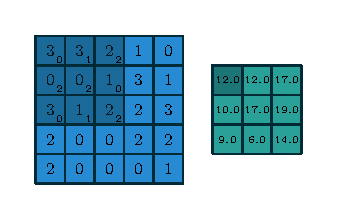
\includegraphics[width=0.7\textwidth]{numerical_no_padding_no_strides_00.pdf}
    \caption[A convolutional operation] {An example of a convolutional
    operation. The image has 5 pixels length and width. The convolutional
    filter has size 3$\times$3. The elements are multiplied together and
    summed to the amount in the top left cell in green. The next step would
    shift the convolutional layer one pixel to the left. For an RGB image, the
    filter would be applied to all three layers. Image source:
    ~\cite{dumoulin2016guide}\label{fig:convolution}}
\end{figure}

To stack layers together for deeper models, there are three  additional core
components. First, to allow the model to find non linear relationships, models
will often include a non linear \textit{activation} function after the
elementwise product and sum operation. Common activation functions include the
\texttt{sigmoid, tanh and ReLU} functions. The \texttt{ReLU} is popular
because it is fast and effective. For an output $x$, the \texttt{ReLU} is
$\max\{0, x\}$.

Second, to reduce the spatial size of the output, a \textit{pooling} layer
reduces a $\ell\times\ell$ patch of the output to a single number. We often
using the $\max$ operator (See Figure~\ref{fig:maxpooling}). Pooling also reduces
the amount of parameters in the model, making it harder for the model to
memorise training data. This is known as \textit{overfitting}, where the model
works well on training data but has poor performance on new data. Pooling
layers act to extract information about what is in the image. The cost of
pooling is that we lose some information about where in the image an object
is. The bulk of a CNN is stacking these convolution, activation and pooling
layers on top of each other.

\begin{figure}
	\centering
    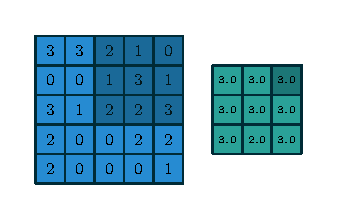
\includegraphics[width=0.7\textwidth]{numerical_max_pooling_02.pdf}
    \caption[A max pooling operation] {An example of a max pooling operation.
    The image has 5 pixels length and width. The pooling filter has size
    3$\times$3. The maximum value of the image within the window is passed to
    the output cell in green. The next step would shift the convolutional
    layer one pixel to the left. Image source: ~\cite{dumoulin2016guide}
    \label{fig:maxpooling}}
\end{figure}

Last, after stacking these layers on top of each other we flatten the
output to a series of dense one dimensional layers. Once we understand these
building blocks, coding them is straight forward (see
Figure~\ref{alg:simple_CNN}).

\begin{figure}
\begin{minted}[
frame=lines,
linenos
]{python}
    # load libraries
from keras.models import Model, Sequential
from keras.layers import Conv2D, MaxPooling2D
from keras.layers import Flatten, Input
from keras.layers import LSTM, Embedding, Dense

model = Sequential()
    # add first convolutional layer with 
    # 64 filters of size 3 x 3
    # and padding to retain image size
    # and ReLU activation function
model.add(Conv2D(64, (3, 3), 
          activation='relu', 
          padding='same', 
          input_shape=(224, 224, 3)))
    # add second convolutional layer with 
    # 64 filters of size 3 x 3
    # and ReLU activation function
    # no padding
model.add(Conv2D(64, (3, 3), 
          activation='relu'))
    # add pooling
model.add(MaxPooling2D((2, 2))
model.add(Flatten())
model.add(Dense(4096, activation='sigmoid')(inputs)
model.add(Dense(10, activation='sigmoid')(inputs)

\end{minted}
    \caption[A simple CNN in\texttt{Keras}]{A simple CNN in\texttt{Keras}. This model
    has two convolutional layers with ReLU activation functions, a max
    poolution layer and a dense layer to predict 10
    classes.\label{alg:simple_CNN}}
\end{figure}
\subsection{Training models}

The question is then: how to train these (hundreds of) millions of parameters?
The high level answer is that we define a \textit{loss function} of the model
error, and try to minimise this function.  The \textit{error} is the
difference between predictions and actual labels and the \textit{loss} is a
differentiable function of the error and the model parameters.

Because the loss function is differentiable, we can use calculus to
approximate the minimum. This step is known as \texttt{gradient descent}.  We
take the gradient of the loss function and update the weights by the negative
of the gradient (see Figure~\ref{alg:graddesc}).  Since we often train on many
thousands (or millions) of images, we cannot compute this in memory. Instead, a
small batch of images is used and the model updated.  This is called
\texttt{batch gradient descent}. There is also stochastic gradient descent for
batches of size one observation. With enough batches, we obtain good results
over time.

\begin{figure}
\begin{minted}
[
frame=lines,
linenos
]{python}
while True:
  weights_grad = evaluate_gradient(loss_fun, 
                                   data, 
                                   weights)
    # perform parameter update
  weights += - step_size * weights_grad
\end{minted}
    \caption[Pseudo code for basic gradient descent]{Pseudo code for basic
    gradient descent. First, we calculate the gradient of the loss function
    with respect to the model weights. We then use this to modify the model
    weights. Source:~\cite{CS231n}\label{alg:graddesc} }
\end{figure}

We don't have to hard code the \texttt{evaluate\_gradient} function, we can
rely on libraries to do this for us. We saw this in Figures~\ref{alg:linreg}
and~\ref{alg:linearimage} above. We have the \texttt{sgd}, or stochastic
gradient descent optimiser and the \texttt{rmse} or root mean squared error
loss function. 

% Some evidence that adaptive weight mechanisms perform better on test set and
% worse on training set (https://arxiv.org/abs/1705.08292). I.e. worse
% generalisation.

There many options for both the optimiser and the loss function. The
development of optimisers is an ongoing area of research
(e.g.~\cite{wilson2017marginal}). Despite the choice, default options will be
 fine for experimentation. Loss functions are selected by the problem
at hand. For regression, root mean squared error loss functions are most
common. For classification, categorical cross entropy is most common. 

These are the simple building blocks for building an object classifier. We now
turn to the literature to understand some important details.

\section{Literature}

The above section is a quick introduction to convolutional neural networks. We
go deeper in this section, focusing on key results in image classification,
object detection and segmentation. These problems nest each other: to detect
an object, a machine needs to output what the object is (classification) and
where it is. To segment and image, the machine needs to output where the object
is (detection and classification) and where the boundaries of these objects
are.

% Measure evolution --> performance on standard tasks

\subsection{Object classification}

Object classification models tell us what is in an image. The output is
a label, for instance a cat or a building. Recent years have seen rapid
evolution in models for classification. We focus on a four key papers that
have defined progress in this field (see Figure~\ref{fig:imagenetoverview}).

\begin{figure}
    \centering
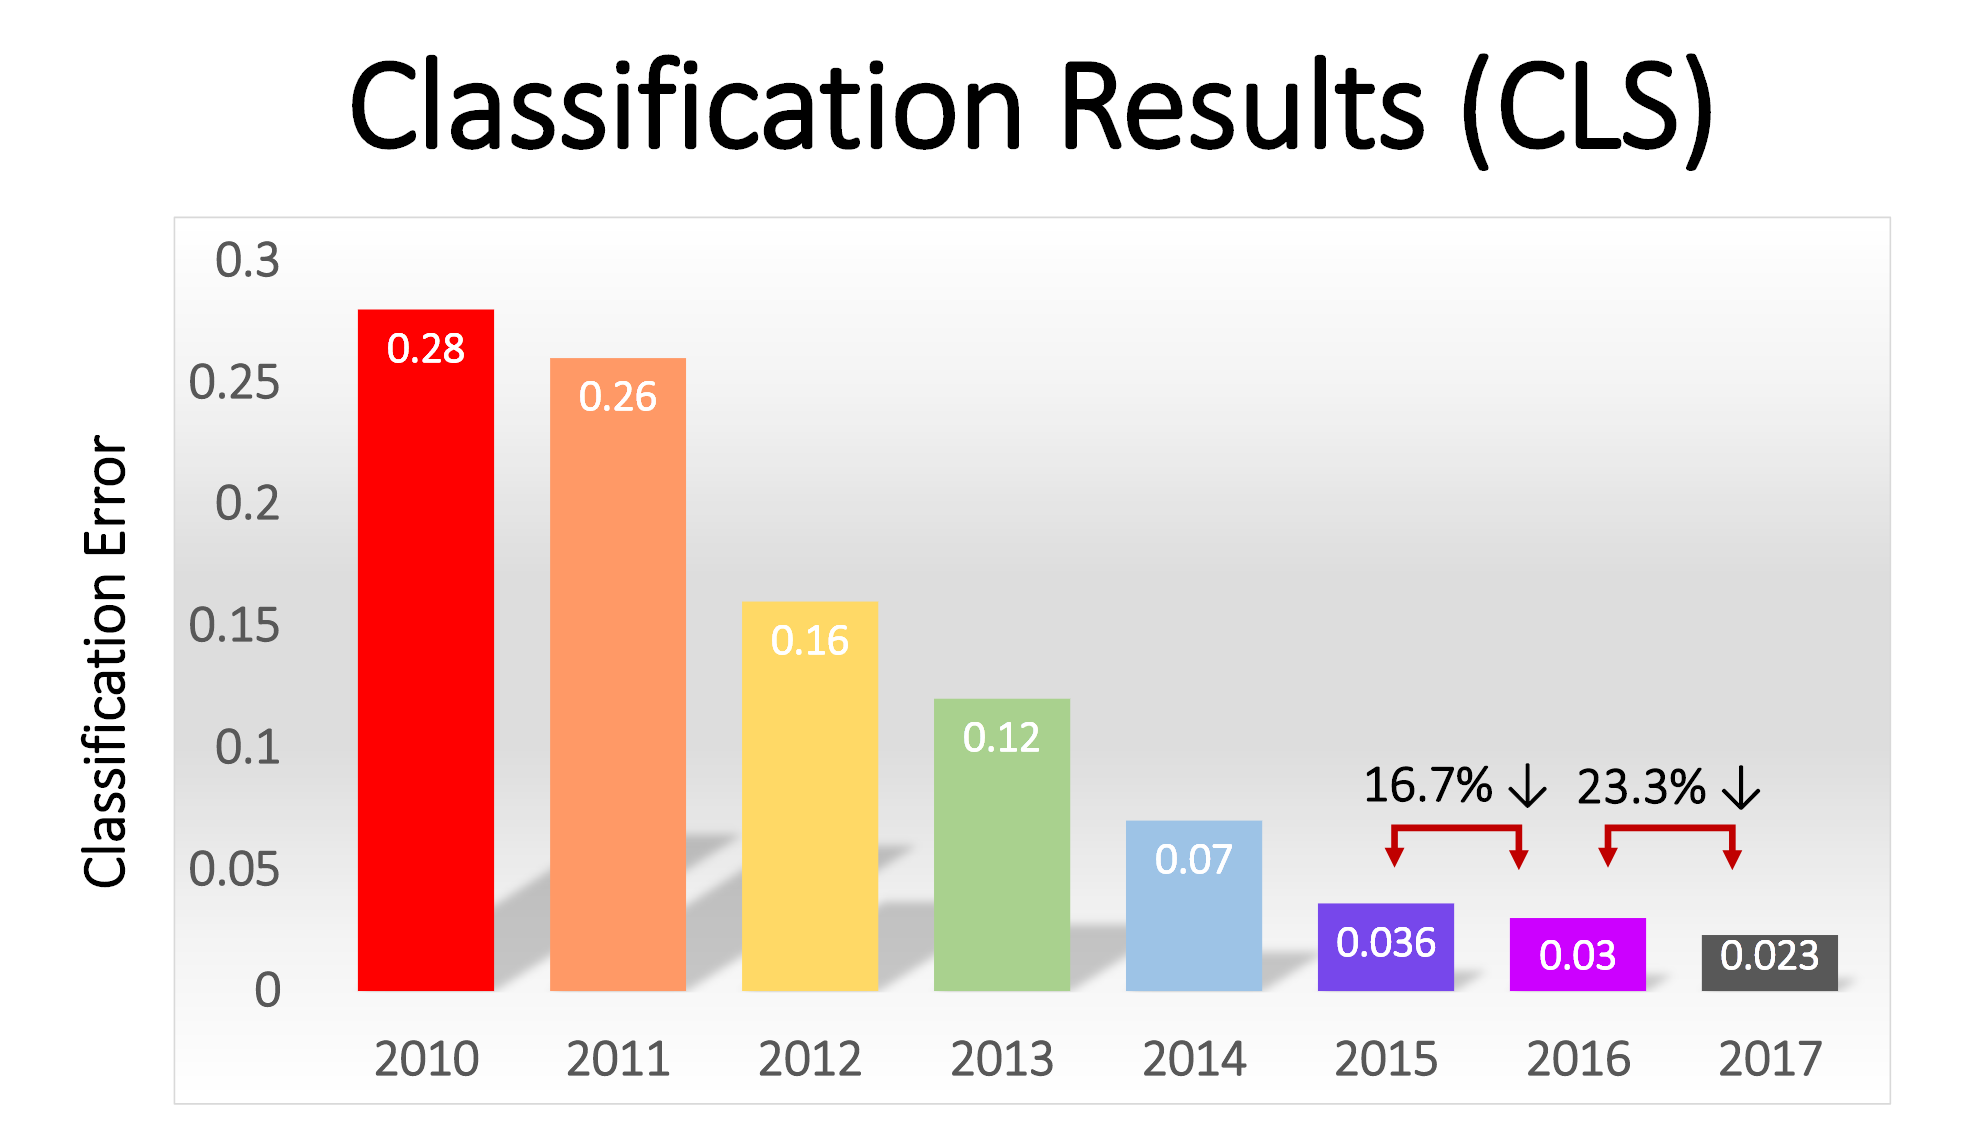
\includegraphics[width=0.7\textwidth]{imagenet_classification_results.png}
    \caption[ImageNet classification results, 2010--2017]{ImageNet
    classification results, 2010--2017. We see that the error rate dropped
    rapidly over 2011--2015. Source: Image Net
    Overivew\footnote{\url{http://image-net.org/challenges/talks_2017/ILSVRC2017_overview.pdf}}\label{fig:imagenetoverview}}
\end{figure}

We begin with AlexNet, which won the ImageNet Classification challenge in
2012~\cite{NIPS2012_4824}.  AlexNet features three innovations which are still
in use today. To begin, AlexNet was the first model to `go deep', with five
convolutional layers.  Second, the model used the \texttt{ReLU} activation
function (discussed above). Last, to prevent overfitting, AlexNet used
dropout. \texttt{Dropout} worked by randomly setting the value of some
parameters to zero during training. This way, the model could not rely on
specific parameters to predict object classes. Instead, the model has to
spread this information across parameters. We can easily add innovations to a
model (E.g., Figure~\ref{alg:dropout}). 

\begin{figure}
\begin{minted}
[
frame=lines,
linenos
]{python}

model.add(Dropout(0.5))
\end{minted}
    \caption[Adding Dropout and ReLU]{Adding dropout to a model is simple.
    Here, we set half of the weights to zero at each training
    iteration.\label{alg:dropout}}
\end{figure}

VGG Net~\cite{SimonyanZ14a} came second in the main image image classification
contest in 2014 (ILSVRC). Although not the best performing model, it has a
simple architecture and is perfect for beginners.  The architecture is a
repeating set of convolutional layers to extract spatial information,
activation layers for non linearities and max pooling to reduce information.

VGG net is widely used as a \textit{feature extractor}. VGG net can extract
features by taking an arbitrary image and setting the output at the flattening
stage. That is, we remove the fully connected layers (or `top') of the model
and reduce the image to a vector. The vector retains some high dimensional
representation of the image that can be used in a standard classifier, for
example a logistic regression model. The original VGG net weights are used,
and no training is undertaken. This common practice can be used to train
models on very few observations.

Models went deeper over the next few years, but a puzzle arose: performance
did not rise -- infact sometimes performance dropped -- with additional
layers. This was a puzzle because models could simply pass on the same output
through multiple layers rather than having degraded performance. This insight
resulted in the residual learning framework that passes both the input $x$ and
the output of a layer $f(x)$ to the next layer. With these skip connections
the model can choose to discard elements of the modified layer output if
elements do not help in prediction. An additional innovation is the lack of
fully connected layers at the end of the model. These innovation allowed
ResNet to have 152 layers and have lower model complexity~\cite{he2016deep}.
ResNet won ILSVRC 2015.

The current state of the art involves creating a model out of an ensemble of
models. The winner of the 2017 ImageNet challenge used ensembles and an
innovation called `Squeeze and excitation'~\cite{wmw}. Squeeze-and-excitation
networks (SENets) weight the information across image channels. That is, if
the red image channel helps with prediction more (say, for fire trucks), the
model will learn to use channel to make predictions. SENets lowered the
ImageNet classification error rate by almost 25 per cent.  

Detecting trucks from cats is a good start, and research is progressing on more
challenging problems. There is still a lot of room to improve for aerial or
satellite imagery. For instance, there is evidence that the number of
satellite bands does not matter for building
detection~\cite{2017Panchromatic}. One needs only layers from the red, green
and blue spectra. One could see SENets exploiting the 5-10 bands of
non visual information that comprise satellite images.

\subsubsection{VGG net in \texttt{Keras}}

In Figure~\ref{alg:vgg} we download the model on line 6. In this block we
download the whole model so that we can use the model to predict what's in the
image. If we want to extract features, we can change the argument
\texttt{include\_top} to be \texttt{False}. Rather than a list of object class
weights, the output of \texttt{model.predict()} will be a 4096 dimensional
vector. We can store these for use in another model.  To date (July 2018),
\texttt{Keras} has ten image classifier models that can be used in the same
way.\footnote{\url{https://keras.io/applications/}}

\begin{figure}
\begin{minted}[
frame=lines,
linenos
]{python}
from keras.applications.vgg16 import VGG16
from keras.preprocessing import image
from keras.applications.vgg16 import preprocess_input
import numpy as np

model = VGG16(weights='imagenet', include_top=True)

img_path = 'remote_area_example.jpg'
img = image.load_img(img_path, target_size=(224, 224))
x = image.img_to_array(img)
x = np.expand_dims(x, axis=0)
x = preprocess_input(x)

features = model.predict(x)
\end{minted}
    \caption[Using VGG16 in \texttt{Keras}]{Using VGG16 in \texttt{Keras}. On
    line 6 we import the model architecture and model weights.\label{alg:vgg}}
\end{figure}

\subsection{Object detection}

The next step after identifying if an object is in an image is pointing out
where the object is. The challenge is to ``detect a \textit{potentially large
number of object instances with varying sizes in the same image} using a
limited amount of computing resources.''~\cite[their emphasis]{NIPS2013_5207}.
Models that solve this problem will be useful for detecting where key sites
--- like damaged roads --- are.

A brute force, basic model is to slide a classifier across an image. Since
this model will have to run multiple times over a single image the model will
be very slow. 

An early innovation is to treat localisation as a regression
problem~\cite{NIPS2013_5207}. This model uses a small standard convolutional
neural network, but instead of a softmax classifier layer, the model uses a
regression layer to output a binary mask: 1 for inside a bounding box, 0 for
outside. One problem was that most of the image is outside the bounding box,
so a model can learn to only output zeros. The authors increase the weights of
non zero outputs to overcome this problem. Overall, there are five networks:
one for box predictions, four others for where the {top, bottom, left, right}
of the box. 

As with many of the models to come, the model in ~\cite{NIPS2013_5207} is
pre-trained on a classification task. A \textit{pre-trained} model is one that
is trained for an additional task, typically where we have lots of data. The
model has then incorporated the capacity to interpret images. This model is
then trained with new data on the task it is required to do, here object
classification. 

The next innovtion came with regions with CNN features
(RCNN)~\cite{Girshick2014, Girshick2015}. RCNN improved the then state of the
art by more than 30\%. Their idea is to extract some two thousand bounding
boxes in a preprocessing step, run a classifier through these boxes and
combine them at the end. They also use supervised pre training on a large
dataset using the VGG net architecture. RCNN works, but is multi stage,
expensive to run and slow. 

Additional innovations increased the speed of this model.
Fast-RCNN~\cite{Girshick2015} shares features across object proposals rather
than recalculating features for each proposal. The model also features a multi
task loss function for classification and a four dimensional regression for
the bounding box. Faster RCNN~\cite{Ren2017} overcomes the bottleneck of
region proposals with a `Regional Proposal Network' (RPN). The RPN takes
\textit{anchors}, or fixed points in the image, and first classifies whether
there is any object there.  Second, the anchor bounding box is adjusted for a
better bounding box fit. FasterRCNN is trainable end to end. This means we can
use gradient descent to train the model all at once, rather than connect
different pieces. 

% \url{https://tryolabs.com/blog/2018/01/18/faster-r-cnn-down-the-rabbit-hole-of-modern-object-detection/}
% Predicing (xmin, xmax, ymin, ymax) is hard. For instance, how to enforce
% xmin < xmax
% Useful overview:
% \url{https://blog.athelas.com/a-brief-history-of-cnns-in-image-segmentation-from-r-cnn-to-mask-r-cnn-34ea83205de4}

% \textbf{Mask RCNN}~\cite{he2017}

% We can do segmentation as well! Have a third branch that allows segmentation. 

% But there is a slight misalignment between bounding boxes and pixels because
% of pixel integers. The original image is say 200 $\times$ 200 and the feature map is
% say 30 * 30. So to select the top 15*15 corner we need 15 * 30 / 200 $\approx$
% 2.25 pixels. RoIPool uses 2$\times$2. RoIAlign (this paper's innovation) uses
% bilinear interpolation to get an idea of what the 2.25th pixel is.


% \textbf{R-FCN}~\cite{NIPS2016_6465}

% The above apply a costly per region subnetwork hundreds of times :(

% \textit{Translation invariance} - the object can be anywhere in an image for
% correct classification

% \textit{Translation variance} - if we move the object, the bounding box should
% change. 

% Use an RPN for proposals.

Despite these innovations, detection was still slow. The You Only Look Once
(YOLO) series of models~\cite{redmon2016yolo} increased the speed of
detection.\footnote{For a video showing the speed at which YOLO can work, see
\url{http://www.youtube.com/watch?v=NM6lrxy0bxs}} YOLO works by dividing an
image into a grid. For each grid cell, there are a fixed number of bounding
boxes. For each bounding box, the model generates five predictions: four
spatial components that modify the shape of a candidate bounding box and a
measure of confidence. The model then applies a classifier. The model uses
Google's LeNet as a base model and shows good performance in new domains. YOLO
version 2 improved performance through pretraining the model on the ImageNet
classification task.

Because of this and the model's speed, YOLO might be useful for a first pass
over large areas of satellite images. One limitation of YOLO is that it is
not the best for identifying many tightly connected objects. To overcome
this and other limitations, a recent paper modifies YOLO for satellite
images~\cite{YOLT}. First, they use upsampling and multiple models at
different scales to capture small images.\footnote{Upsampling is discussed
below} For instance, one classifier for airports and another for airplanes.
Second, they define a new network architecture with a denser final output for
smaller bounding boxes.

\subsection{Image segmentation}

The final task we investigate is image segmentation. The challenge here is to
outline the boundary of the object (see Figure~\ref{fig:segmo}). In one sense this is a
simple extension of classification: but one prediction per pixel rather than
one prediction per picture. Segmentation would be useful in tracing out road
paths and distinguishing regions with damaged properties versus non damaged. 

\begin{figure}
    \centering
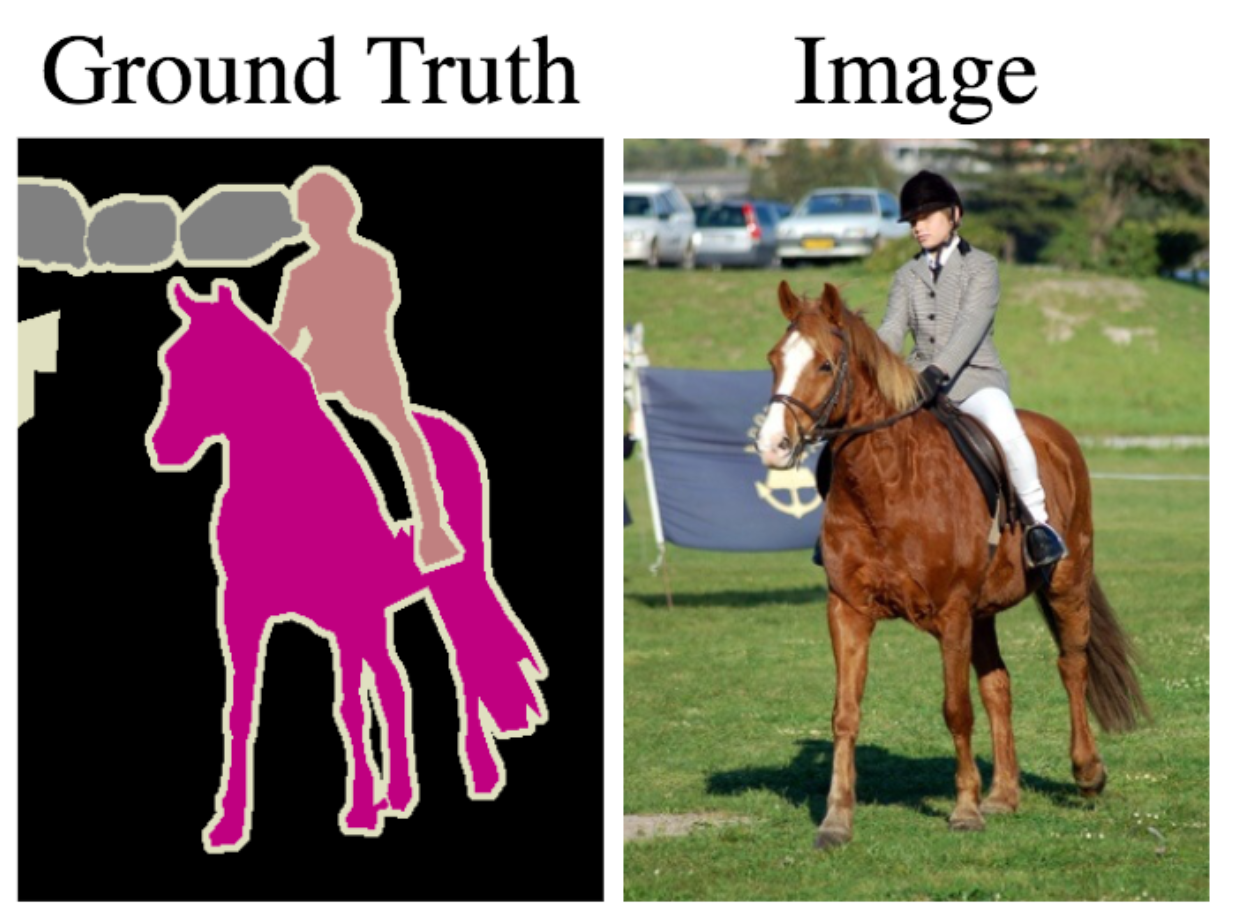
\includegraphics[width=0.5\textwidth]{Figures/segmentation-example.png}
\caption[An example of an image segmentation problem]{An example of an image
    segmentation problem. The model must predict the horse, the rider, the
    three cars and the boundaries between them. Source:~\cite{long2015fully}
\label{fig:segmo}} \end{figure}

% In fact, early models ran a class model over each pixel~\cite{NIPS2015_5852}. 
With segmenation, there is a tension between semantics and location.
\textit{Semantics} is the question of what, \textit{location} asks where.
Local information helps answer the former and global information helps answer
the latter. This need for two types of information gave rise to complicated
models prior to the era of fully end to end differentiable models. This
tension also explains the innovations beyond basic CNNs used for
classification.

\cite{long2015fully} developed the first end to end trained CNN for
segmentation. \cite{long2015fully}'s insight was to think of
a fully connected layer as a 1 x 1 convolutional layer that covers the whole
image. Using a standard CNN (e.g. VGG net) did not work well as by the
time you've gotten to predicting a pixel, you've lost a lot of the information
on the surrounding pixels. The authors get around this by bringing
intermediate layers back into the prediction (Figure~\ref{fig:skipsegmo}).
This allowing the model to combine coarser semantic information and finer
appearance information. 

\begin{figure}
    \centering
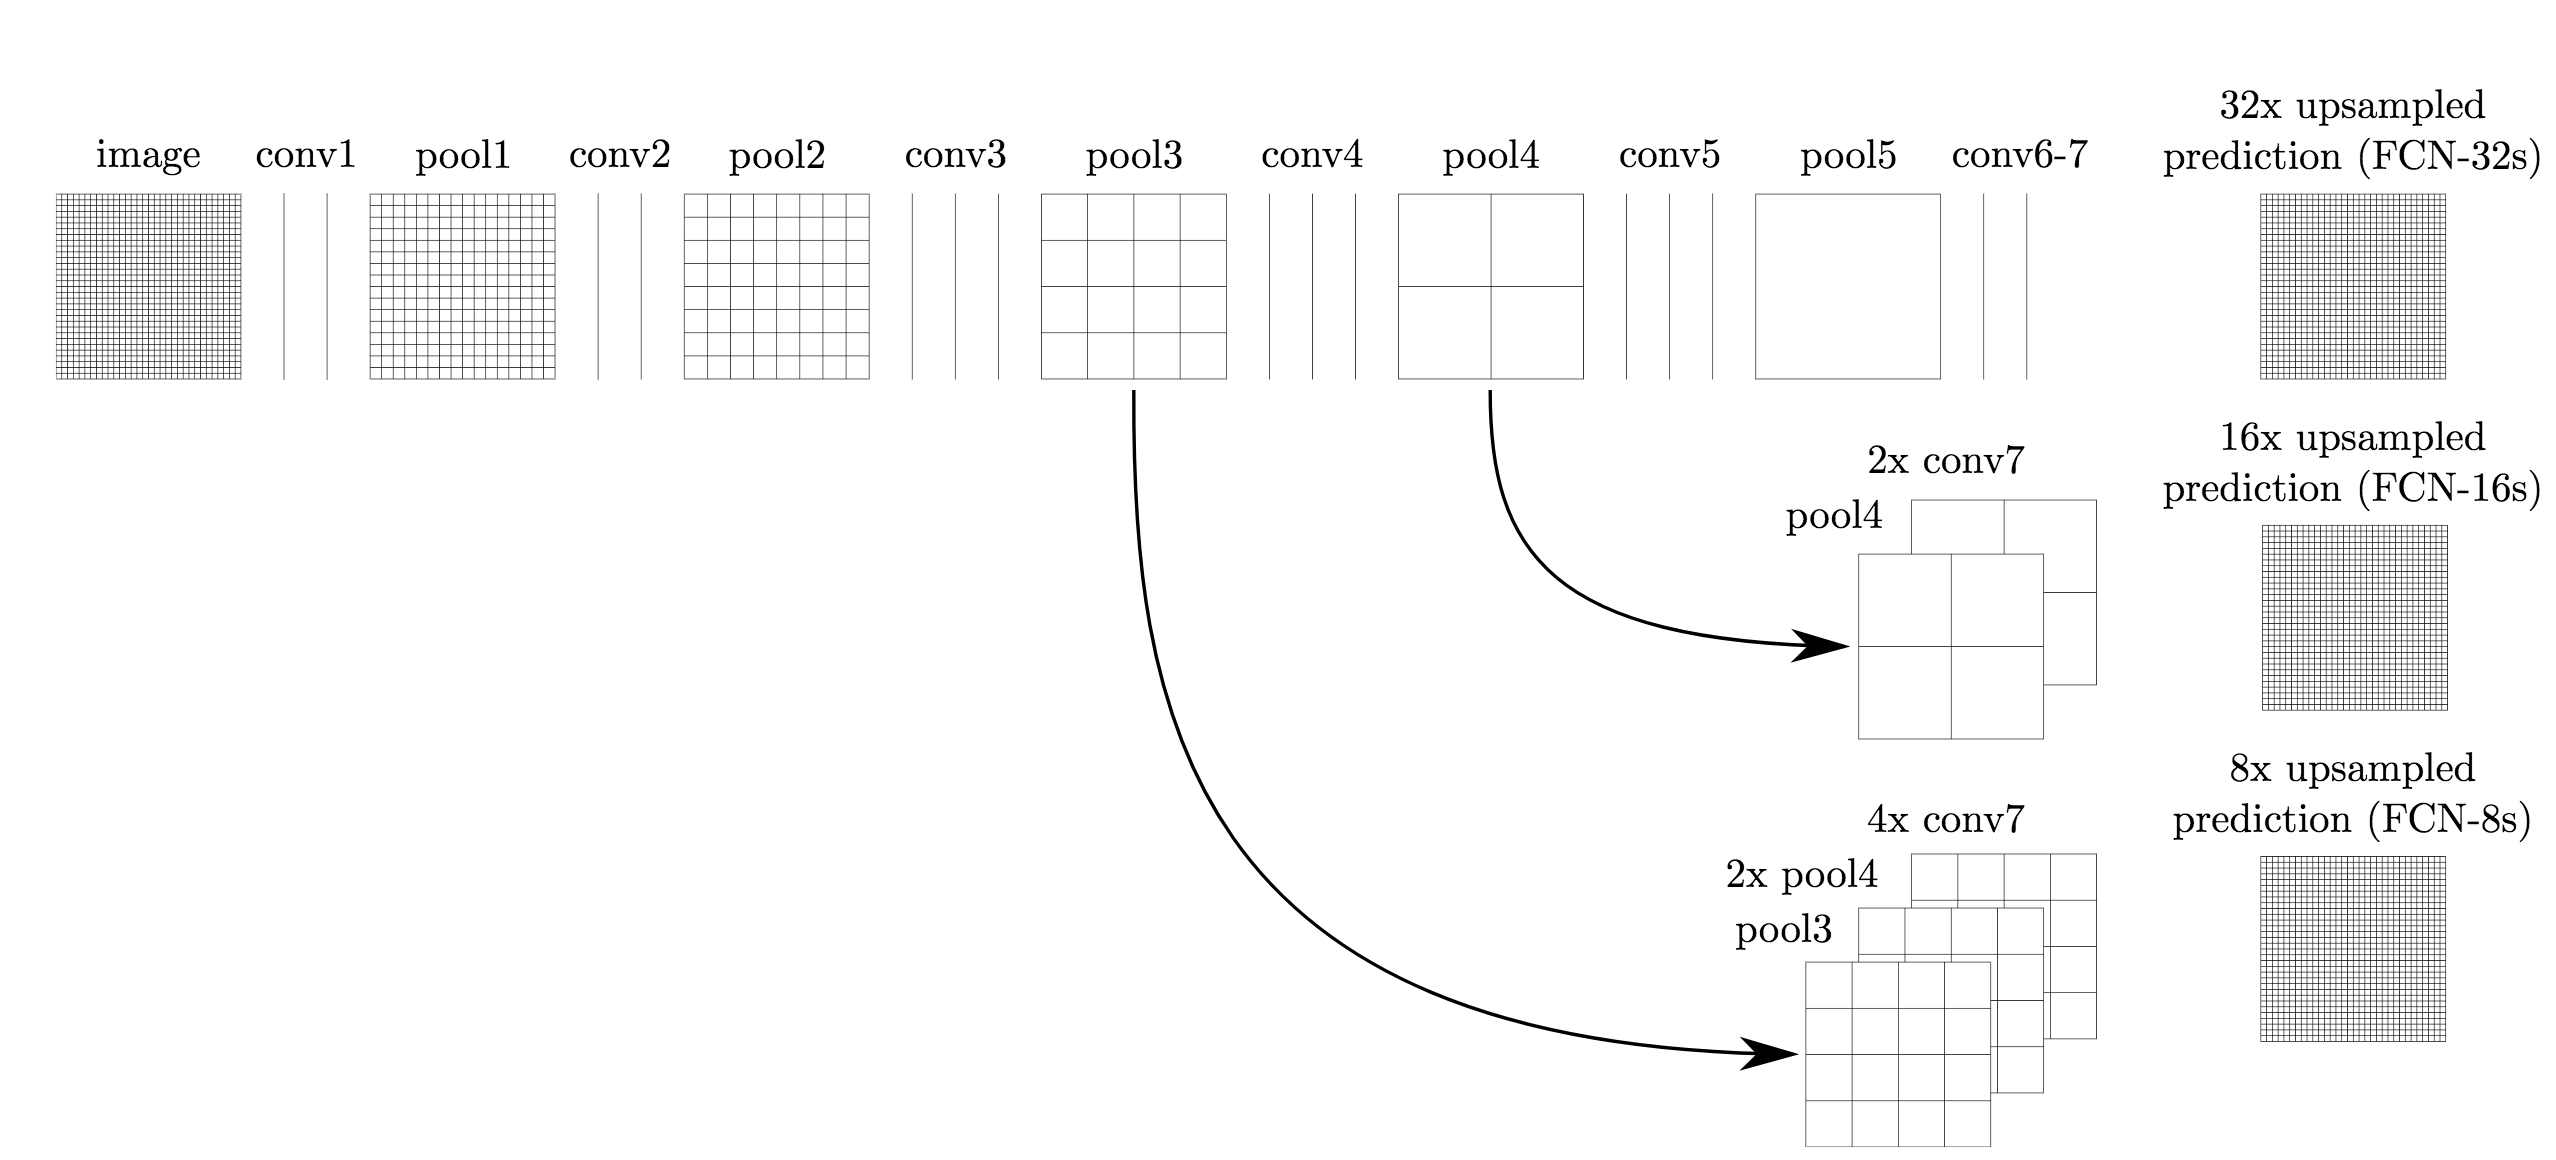
\includegraphics[width=0.75\textwidth]{Figures/skip-segmentation.png}
    \caption[Skip architecture for segmentation]{Skip architecture for
    segmentation. Output from the Pool3 and Pool4 are combined with outputs of
    Conv7 for more refined location predictions.
    Source:~\cite{long2015fully}\label{fig:skipsegmo}}
\end{figure}

The output of this model was still too coarse. The solution was to bring in more
skips. Many models do this~\cite{segnet, unet}.\footnote{If you like, you can
always combine the two~\url{https://github.com/ykamikawa/Seg-UNet}}
U-Net~\cite{unet} uses a CNN to \textit{encode}, or extract features. A
\textit{decoder} network then converts these features into a per pixel
classification. Because the feature is a small dense representation, the
decoder network must \textit{upsample} -- or `blow up' -- the image from the
dense representation. A benefit of UNets is that we can use any pretrained
network to encode the data. UNets are commonly used in the data science
community. Segnet uses a similar architecture, but uses less computational
space to do so.

An alternative attack on using both local and global information is to discard
max pooling and use components that compress class information while retaining
location info~\cite{chen2018,dilated2017}. These components, called
\textit{atrous} convolutions, generate low to mid resolution outputs
(Figure~\ref{fig:dilation}).  Models using atrous convolutions require an
additional step to refine the segmentation. Conditional Random Fields (CRF)
are used most often.

\begin{figure}
    \centering
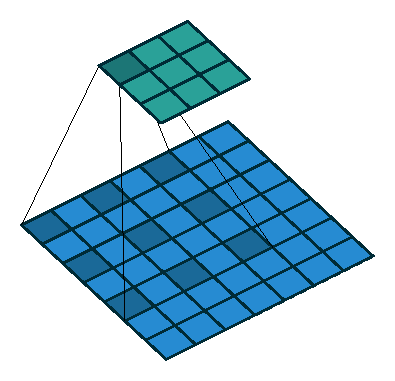
\includegraphics[width=0.7\textwidth]{conv_arithmetic/pdf/dilation_00.pdf}
    \caption[Dilation]{Dilation operation
    Source:~\cite{dumoulin2016guide} \label{fig:dilation}} 
\end{figure}

Mask RCNN~\cite{he2017} extends faster RCNN by adding a branch to the model
for pixel level classification.  Since the output of the CNN is smaller than
the ground truth image, some form of \textit{upsampling} or increasing the
size of output images is required.  Mask RCNN achieves this by using
interpolation. Say our image size is 512 x 512, we are proposing a region in
the top left 25 x 25 pixel corner, and feature map is size 30 x 30. Then our
region of interest is 25 $\times$ 30 / 512 $\approx$ 1.46 pixels of the
feature map. A naive implementation would use integer division for a region
proposal of 1 pixel. Mask RCNN uses bilinear interpolation to estimate what
the 1.46th pixel would look like.

% outputs. A

% Repeated pooling shrinks output size. Long range skip connections. Use
% \textit{chained residual pooling} which  is  able  to  capture
% background context from a large image region. It does so  by  efficiently
% pooling  features  with  multiple  window sizes and fusing them together with
% residual connections and learnable weights

% \paragraph{Learning to segment object candidates}~\cite{NIPS2015_5852} 

\section{Analysis with satellite images}

We now look some practical applications with satellite images. There are three
branches of knowledge we can look at. First, there is the academic literature.
Second, data science competitions. Last, we have industry.

\subsection{Applications in academia}

Much of the academic literature takes a pre-trained CNN or common
architecture and trains the model on the task at hand. Two papers have focused
on mapping poverty~\cite{babenko2017poverty,Jean79}. \cite{babenko2017poverty}
use satellite images, land use maps and household survey data to map
poverty in Mexico.  They trained a model using RGB bands and near infrared
band.  Because pretrained models use the three RGB bands, the model had to be
retrained from scratch to exploit all satellite bands.  Around fifty per cent
of variation in local poverty can be predicted through satellite images and a
CNN alone. This increases to around sixty per cent when they include land use
cover as a feature. It is not clear from the paper how they include land use
cover information maps. It does not seem to be a feature layer, perhaps it was
used as a regression input with the CNN output, see (1).

\begin{equation}
\textup{composite prediction} = \alpha + \beta\textup{CNN output} + \phi\textup{land use}
\end{equation}

\cite{Jean79} estimate poverty across Sub Saharan Africa. Since ground truth
values are difficult to come by, they use night lights as a proxy. They fine
tune a pretrained CNN (VGG 8 layer) to predict night lights. These
features are fed into a ridge regression model (LASSO) to estimate poverty
taken from household surveys. The satellite data is taken from the Google
Static Maps API. Pixels are approximately 1km square. The model's transfer
learning is promising. Figure~\ref{fig:transfer} shows the average $R^2$ for
models trained on one country and evaluated each country.

\begin{figure}
    \centering
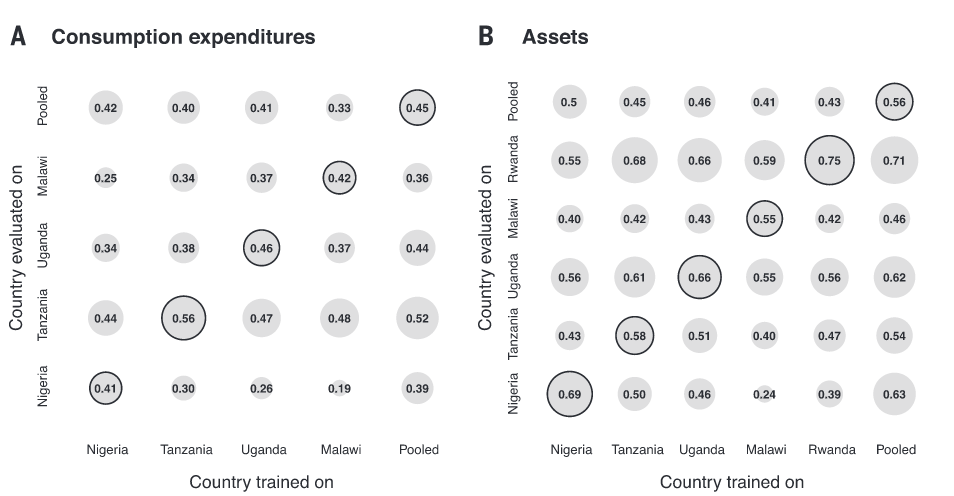
\includegraphics[width=0.7\textwidth]{transfer-learning-poverty.png}
    \caption[Transfer learning for CNNs used for poverty
    estimation]{Understanding how well models trained on satellite images from
    one country generalise to another country. Source:~\cite{Jean79}\label{fig:transfer}}
\end{figure}

A similar strand of research maps population~\cite{doupe2016, robinson2017}.
\cite{doupe2016} map population in Kenya and Tanzania using a VGG-net style
architecture. The authors exploit all eight landsat bands by retraining a
model from scratch. \cite{robinson2017} also train their
own model. They use a two step procedure to obtain raw estimates for
population. The first gets coarse values at the pixel level. These are
combined at the county level. The results are directly interpretable as
population estimates. Facebook~\cite{facebook} are also estimating
population. This seems to be a building segmentation map. Local population
density is estimated by taking the known population and spreading this
population amongst the area inferred from the building segmentation map.  In
addition, Facebook use segmenting tools to identify roads~\cite{demir2018}.

\subsection{Applications in the data science community}

In the past few years, data science
competitions have been organised around small, high resolution datasets. The
two SpaceNet challenges asked participants to segment roads, buildings and
water bodies, amongst others.

In the first edition, the test challenge was to predict buildings in Rio de
Janiero, Brazil. This is particularly challenging because buildings in Rio are
small and densely built. Four of the top five entries used CNNs. Second
place used SSD, third MNC whereas forth and fifth trained their own model.
Fifth place in particular placed a large emphasis on image augmentation. The
winner used a sequence of well trained random forest models.

In the second edition, additional cities were added. These cities (Las Vegas,
Paris, Shanghai and Khartoum) all have a different built infrastructure. The
winner used U-Net. To use all the spectral bands, the model had to be trained
from scratch. This model did struggle with small and L shaped buildings. The
second and third places used models based on the chained random forests models
that won the first edition. 

Last, we note that there is a new competition
that is worth keeping your eyes on\url{http://deepglobe.org/challenge.html}.

\subsection{Applications in industry}

Many industries use satellite data to generate information. We do not have
access to proprietry methods; however, understanding applications may assist
in generating ideas. Common applications include crop monitoring and
forecasting,\footnote{\url{https://telluslabs.com/}} water cover and
use,\footnote{\url{https://www.vandersat.com/}} car park occupancy rates
(consumer demand) and oil
reserves\footnote{\url{http://www.orbitalinsight.com/}}. Of note is the
insurance industry, who use satellite images for predicting claims amounts,
and identifying damaged or unaffected assets. As one would expect, the
intelligence community and associated research groups are doing work
too.\footnote{For instance, CosmiQ
(\url{http://www.cosmiqworks.org/space-30/}) have developed a time series
model to map infrastructure after a hurricane~\cite{cosmiq} and a tool to
create your own time series from satellite
imagery~\url{https://github.com/CosmiQ/CometTS}}

\subsection{NGO applications}


NGOs have tended to use traditional GIS technolgoies --- like change detection
--- to identify damaged buildings. For instance, HRW used before and after
photos to identify burned buildings in Rohingya villages throughout
Burma~\cite{2016Burma}. Amnesty International used
satellite images to identify buildings and villages attacked by Boko Haram in
Nigeria~\cite{2015Nigeria}. Other applications include identifying the 2011 Oil Spill in
Niger~\cite{Koettl2011} and mass graves in Afghanistan~\cite{2013AAAS}. A key
aspect of these is that the locations were roughly known prior to analysis.
For more applications, see~\cite{2014Human}. 

\section{Satellite data}

There are many sources of satellite imagery.\footnote{The following URLs
provide a good list as of July 2018:
\url{https://gisgeography.com/free-satellite-imagery-data-list/}}
% \url{https://docs.google.com/spreadsheets/d/1oFY_TX5QRFyAAu-nxeClnOFB1epSlSDWEHoMalvv0Qs}}
Satellite imagery is expensive, but free or limited options are available. For
isntance, both LANDSAT and the Copernicus mission images are free of charge and
available through the USGS Earth
Explorer\footnote{\url{https://earthexplorer.usgs.gov/}} and the Scientific
Data Hub\footnote{\url{https://scihub.copernicus.eu/dhus/}} or the
Google Earth Engine.\footnote{\url{https://earthengine.google.com/}} LANDSAT
has the benefit of a forty year history of images, although at 30m (15m
panchromatic) the resolution is course. The Copernicus Programme's Sentinel
satellites have a resolution of 10m. At these resolutions, individual
buildings will be difficult to isolate.

We know that image resolution matters~\cite{2017The}. It is difficult with the
naked eye to locate a 10 square meter building with 10 square meter pixels.
For the most part, higher resolution imagery typically costs money. For
humanitarian and research purposes, small datasets can be provided. For
instance, Planet and Satellogic have researcher and humanitarian
access~\cite{Planet,Satellogic}. I would not be surprised if other providers
matched this offer. In addition, Google maps and Bing Maps have APIs that
allows users do download a limited amount of  undated high resolution images.
The images have a watermark which can easily be cropped out.
Table~\ref{tab:meinetabelle} presents an overview of high resolution image
providers.

\begin{table}[htb]
\caption{A list of satellite imagery providers}
\begin{tabular}{lcr}
Provider & Free & Description \\
\hline
    Planet & Limited & 3--5m imagery anywhere in the world \\
    Satellogic & Limited & 30 bands, 30m resolution \\
    UrtheCast & N & 0.75m resolution, video available \\    
    Digital Globe & N & Global coverage, 30 cm resolution \\ 
    Bing & Y & High resolution, undated \\
    Google & Y & High resolution, undated \\
\end{tabular} 
\label{tab:meinetabelle}
\end{table}

\subsection{Labelled data}

Training models requires labelled data. One option is to do this by hand or
outsource to services like Mechanical
Turk.\footnote{\url{https://www.mturk.com/}} For drone data or specific
objects to detect, this is a good option. For buildings, roads or waterways,
there are a few datasets of use. Some of these are down, but may still be
available through other researchers, or asking the organisers.

First, there is the Spacenet challenge
data.\footnote{\url{https://spacenetchallenge.github.io/datasets/datasetHomePage.html}}
This data appears to be down at present. The data consists of very high
resolution (30--50cm) images of five cities. The data contains labels of
buildings, trees, cards, roads and waterways. More labelled urban environments
can be found in Urban Environment
dataset.\footnote{\url{https://github.com/adrianalbert/urban-environments/tree/master/dataset-collection}}
For labels, there are two good sources. First, the Urban Atlas
project.\footnote{\url{https://www.eea.europa.eu/data-and-maps/data/copernicus-land-monitoring-service-urban-atlas}}
This project is used in the Urban Environment dataset. A second option is
OpenStreetMap.\footnote{\url{https://www.openstreetmap.org}} These maps are
created by volunteers, much like wikipedia. Your mileage may vary with
building accuracy. 

\section{Conclusion}

Deep learning is made rapid progress in the ability of computers to extract
information from images. In addition, recent advances in satellite technology
have allowed companies to provide timely, high quality satellite images. These
images can provide large amounts of information for understanding how nature
and society is changing on the ground. We can harness two developments to
understand what is happening in the immediate aftermath of a disaster.
 
This report has attempted to provide a high level overview to deep learning
for satellite imagery. We presented the ideas behind models that can tell us
what is in an image and where in the image an object is. 
We connected these ideas to \texttt{Python} code, so that the reader can
understand how to implement these in practice. Although there is a little more
to building models than in this report, these code fragments provide the basis
for understanding the vast array of available blog posts, tutorials and MOOCs.
Last, we present applications and data sources.


%----------------------------------------------------------------------------------------
%	BIBLIOGRAPHY
%----------------------------------------------------------------------------------------

\renewcommand{\refname}{\spacedlowsmallcaps{References}} 

\bibliographystyle{unsrt}

\bibliography{review.bib}

%----------------------------------------------------------------------------------------

\end{document}
